\documentclass[12pt]{article}

\usepackage[utf8]{inputenc}
\usepackage{fancyhdr}
\usepackage{graphicx}
\usepackage{amsmath}

\pagestyle{fancy}
\fancyhead[L]{Jeppe Møldrup}
\fancyhead[C]{Matematik 18}
\fancyhead[R]{30/04-2019}

\title{Matematik aflevering 18}
\author{Jeppe Møldrup}
\date{}

\begin{document}

\maketitle

\section*{Opgave 9}

\begin{enumerate}

        \item[a.] Bestem $\angle A$, og bestem arealet af trekant $ABC$

                Vi kender siderne a og c og vinklen mellem dem.
                Arealet af en trekant er givet ved
                $$T=\frac{1}{2}ab\cdot \sin (C)$$
                Så vi indsætter
                $$T=\frac{1}{2} \cdot 94\cdot 58\cdot \sin (89)=2725.58$$
                finder A ud fra cosinusrelationen
                $$b = \sqrt{a^2 + c^2 - 2ac\cdot \cos (B) } \Leftrightarrow b=109.59$$
                $$A = \cos ^{-1} (2725.58/(0.5\cdot 58\cdot 109.59)) = 59.05^{\circ}$$
                Så vinkel A er $59^{\circ}$

        \item[b.] Bestem længden af medianen fra $A$ på siden $a$

                [Indsæt billede]
                Punktet D ligger på medianens skæringspunkte, og derfor er siden $|BD|=\frac{a}{2}$
                Jeg bruger cosinusrelationen der er
                $$a^2=b^2+c^2-2ab\cdot \cos (C) \Leftrightarrow |AD|=\sqrt{47^2+58^2-2\cdot 47\cdot 58\cdot \cos (89)}=74.01$$
                Så Længden af medianen er 74

\end{enumerate}

\section*{Opgave 10}

\begin{enumerate}

        \item[a.] Bestem en ligning for tangentil til grafen for funktionen $f$ givet ved
                $$f(x) = (x^2 + 5x + 500)\cdot e^{\frac{-x}{100}}$$
                i punktet $P(0, f(0))$

                Jeg starter med at finde den korrosponderende $y$-værdi til punktet $P$
                $$f(0) = 500$$
                Så punktet $P$ er $(0, 500)$. Så differentierer jeg $f$
                $$f'(x) = (39x\cdot 20^{-1}-x^2\cdot 100^{-1})\cdot e^{-x\cdot 100^{-1}}$$
                Så finder jeg hældningen af grafen i punktet $P$ idet det er
                tangenhældningen
                $$a = f'(0) = 0$$
                Så tangentens ligning er
                $$y = 0x+b$$
                Så indsætter jeg punktet $P$ ind i ligningen
                $$500 = 0\cdot 0 + b \Leftrightarrow b = 500$$
                Så tangentens ligning er
                $$y = 500$$

        \item[b.] Bestem monotoniforholdene for $f$, og tegn grafen for $f$ i et
                passende vindue

                For at bestemme monotoniforholdene finder jeg alle mulige
                ekstremaer, dvs. punkter hvor $f'(x) = 0$ vha. solve.
                $$solve(f'(x) = 0,x) \rightarrow x = 0 \vee x = 195$$
                Så kigger jeg på områderne før, efter og mellem punkterne for
                at finde ud af om de er maksimummer, minimummer eller
                vandrette vendetangenter
                $$f'(-1) = -1.98$$
                $$f'(1) = 1.92$$
                $$f'(200) = -1.35$$
                Så kan monotonilinjen tegnes
                \begin{center}
                        \begin{tabular}{c | c c c c c}
                                $x$ & & 0 & & 195 & \\ \hline
                                $f'(x)$ & - & 0 & + & 0 & - \\
                                $f(x)$ & $\searrow$ & lok. min. & $\nearrow$ & lok. max. & $\searrow$ \\
                        \end{tabular}
                \end{center}
                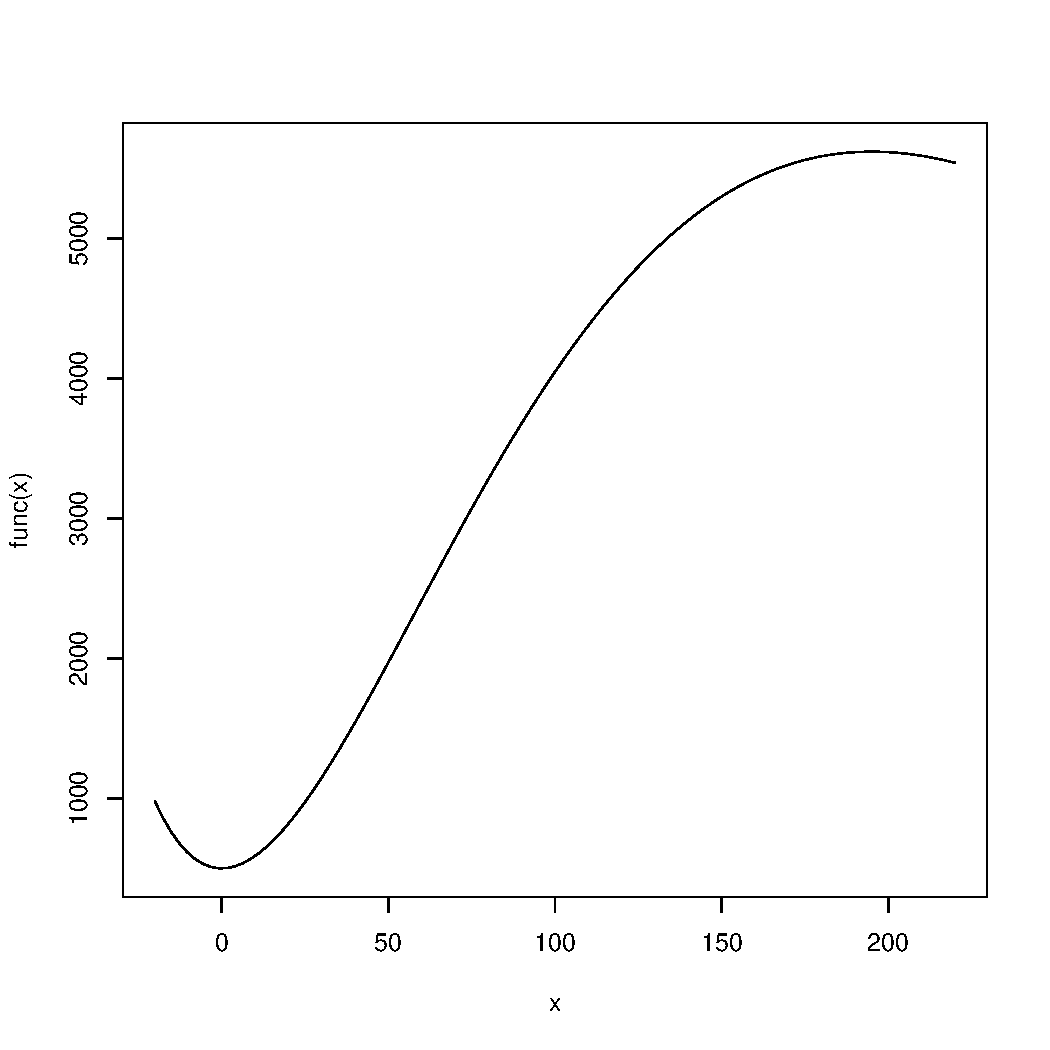
\includegraphics[width=\textwidth]{dia/10b.pdf}

\end{enumerate}

\section*{Opgave 11}

\begin{enumerate}

        \item[a.] Benyt modellen
                $$c(x) = \frac{12500\cdot x-2500\cdot x^2}{150+7.8^x}+90,~~~~0\le x\le 7$$
                til at bestemme det tidspunkt, hvor glukosekoncentrationen i
                personens plasma er maksimal

                Jeg finder alle punkter hvor $c'(x) = 0$, dvs. alle mulige
                ekstremaer
                $$solve(c'(x) = 0,x) \rightarrow x = 1.61955 \vee x = 5.53478$$
                Så kigger jeg på områderne før, efter og mellem for at se
                om det er maksimummer, minimummer eller vandrette vendetangenter
                $$c'(1) = 41.0941$$
                $$c'(2) = -30.3123$$
                $$c'(6) = 0.0589824$$
                Så vi ved at ved $x = 1.62$ er der et maksimum. men grafen stiger
                også efter $x = 5.53$ så jeg kigger på ved om $x = 7$ for at se
                om det er højere end $x = 1.62$
                $$c(1.62) = 166.959$$
                $$c(7) = 89.9801$$
                Her kan jeg se at ved $x = 1.62$ ligger højere end $x = 7$
                Så det er maksimummet.

        \item[b.] Benyt modellen til at bestemme, hvor lang tid glukosekoncentrationen
                i personens plasma ligger over 130 mg/dl.

                Jeg finder alle punkter hvor $c(x)$ skærer $y = 130\ mg/dl$ vha. solve
                $$solve(c(x) = 130,x) \rightarrow x = 0.5505316 \vee x = 2.665899$$
                Jeg tager så de to tidspunkter og finder ændringen i tid, dvs.
                hvor lang til koncentrationen er over 130 mg/dl. Jeg ved at
                koncentrationen er over 130 i dette område idet maksimummet
                fra sidste opgave ligger mellem de to punkter
                $$\Delta x = 2.665899-0.5505316 = 2.1153674$$
                Så koncentrationen af glukose ligger over 130 mg/dl i 2.12 timer.

\end{enumerate}

\section*{Opgave 12}

\begin{enumerate}

        \item[a.] Bestem volumen af det omdrejningslegeme, der fremkommer,
                når $M$ drejes $360^{\circ}$ omkring førsteaksen

                Jeg bruger formlen for volumnet af omdrejningslegeme
                $$V = \pi \int_a^b (f(x))^2\ dx$$
                Så jeg indsætter
                $$V = \pi \int_0^4 (x^3-6x^2-32)^2\ dx = 4779.52$$
                Så volumen af omdrejningslegemet er 4779.52

        \item[b.] Bestem forholdet mellem arealerne af $M$ og $N$.

                For at finde forholdet mellem arealerne, skal jeg have en formel for
                begge arealer. Arealet $M$ findes
                $$T = \int_0^4 f(x)\ dx$$
                Arealet af $N$ findes ved at finde arealet under $y = 32$ fra 0 til 6
                og trække arealet under $f(x)$ mellem 0 til 6 fra. dvs.
                $$T = \int_0^6 y(x)\ dx - \int_0^6 f(x)\ dx$$
                Så finder jeg forholdet
                $$\frac{\int_0^4 f(x)\ dx}{\int_0^6 y(x)\ dx - \int_0^6 f(x)\ dx} = 0.59$$
                Så forholdet mellem dem er 0.59, dvs.
                $$M = 0.59\cdot N$$

\end{enumerate}

\section*{Opgave 13}

\begin{enumerate}

        \item[a.] Opstil en nulhypotese, der passer til forsøget, og bestem de
                forventede værdier.

                \begin{center}
                        \begin{tabular}{c | c | c | c}
                                & fork & ikke fork & sum \\ \hline
                                kold &&& 90 \\ \hline
                                ikke kold &&& 90 \\ \hline
                                sum & 18 & 162 & 180 \\
                        \end{tabular}
                \end{center}

                Jeg opstiller nulhypotesen $H_0$: Forkølelse er uafhængig af kolde
                fødder.

                Jeg udregner de forventede værdier med formlen
                $$Rækkesum\cdot \frac{Kolonnesum}{totalsum}$$
                F.eks folk med kolde fødder der fik forkølelse
                $$90\cdot \frac{18}{180} = 9$$
                Så får jeg tabellen
                \begin{center}
                        \begin{tabular}{c | c | c | c}
                                & fork & ikke fork & sum \\ \hline
                                kold &9&81& 90 \\ \hline
                                ikke kold &9&81& 90 \\ \hline
                                sum & 18 & 162 & 180 \\
                        \end{tabular}
                \end{center}

        \item[b.] Undersøg, om nulhypotesen kan forkastes på et 5\% signifikansnivau.

                13 folk med kolde fødder fik forkølelse. Så jeg udregner de andre
                via summene
                \begin{center}
                        \begin{tabular}{c | c | c | c}
                                & fork & ikke fork & sum \\ \hline
                                kold &13&77& 90 \\ \hline
                                ikke kold &5&85& 90 \\ \hline
                                sum & 18 & 162 & 180 \\
                        \end{tabular}
                \end{center}
                Så kører jeg en $\chi^2$ uafhængighedstest på tabellen for
                at se om den passer med min $H_0$\\
                Jeg får resultatet
                $$\chi^2 = 3.95~~~~p-value=0.0469$$
                Idet p<0.05 skal $H_0$ forkastes.
                Så det betyder at forkølelse er afhængig af kolde fødder.

\end{enumerate}

\section*{Opgave 14}

\begin{enumerate}

        \item[a.] Bestem en forskrift for $V$, og bestem personens vægt 45 dage
                efter slankekurens start.
                $$\frac{dV}{dt} = \frac{1}{7700}(D-40\cdot V)$$
                Jeg finder løsningen til differentialligningen vha. desolve jeg
                ved at han starter ved 95 kilo til $t = 0$ og hans daglige
                kalorieindtag er 2800 kcal.
                $$desolve(V'=7700^{-1}(2800-40V) and V(0) = 95,V,t) \rightarrow
                V(t) = 25\cdot e^{-2t\cdot 385^{-1}}+70$$
                Så indsætter jeg 45 ind i funktionen for at finde hans vægt
                efter 45 dage.
                $$V(45) = 89.79$$
                Så efter 45 dage vejer han 89.79 kilo.

        \item[b.] Benyt modellen til at bestemme, hvor stort denne persons
                daglige energiindtag skal være, for at ønsket kan opfyldes.

                Personen vejer 100 kg, og ønsker at tabe 5 kilo efter 90 dage.

                Jeg finder $D$ til tidspunktet $V(90)=95$ vha. solve
                $$solve(V(90) = 95,D) \rightarrow D = 3464.46$$
                Så hvis personen vil nå sit mål skal de indtage
                3464.46 kcal om dagen.


\end{enumerate}

\section*{Opgave 15}

\begin{enumerate}

        \item[a.] Gør rede for, at $\alpha$ er bestem ved ligningen $x+2y+z=9$

                Jeg starter med at finde normalvektoren til $\alpha$ ved
                at finde krydsproduktet mellem vektoren fra A til B
                og vektoren fra A til C. Krydsproduktet ligger ret på de to vektorer
                og alle punkter ligger i planen så derfor ligge krydsproduktet ret
                på planen og er derfor en normalvektor
                $$\vec{AB} = \begin{pmatrix} 1-0 \\ 4-3 \\ 0-3 \end{pmatrix}
                        = \begin{pmatrix} 1 \\ 1 \\ -3 \end{pmatrix}$$
                $$\vec{AC} = \begin{pmatrix} 6-0 \\ 0-3 \\ 3-3 \end{pmatrix}
                        = \begin{pmatrix} 6 \\ -3 \\ 0 \end{pmatrix}$$
                $$crossp(\vec{AB}, \vec{AC}) = \begin{pmatrix} -9 \\ -18 \\ -9 \end{pmatrix}$$
                        Jeg kan forkorte krydsproduktet med -9, så jeg får
                $$\vec{n_{\alpha}} = \begin{pmatrix} 1 \\ 2 \\ 1 \end{pmatrix}$$
                Så indsætter jeg den og punktet A ind i planens ligning
                $$a(x-x_0)+b(y-y_0)+c(z-z_0)=0$$
                $$(x-0)+2(y-3)+(z-3) = 0$$
                $$x+2y+z-9=0$$
                $$x+2y+z=9$$
                Så de er ens.

        \item[b.] Bestem $k$ så $l$ ligger i planen

                $$l:~~~~\begin{pmatrix} x \\ y \\ z \end{pmatrix} =
                        \begin{pmatrix} 0 \\ 3 \\ 3 \end{pmatrix} +
                        t \cdot \begin{pmatrix} 3k \\ 1 \\ -k \end{pmatrix}$$
                Hvis linjen skal ligge i planen, skal linjen ligge ret på 
                planens normalvektor, dvs. prikproduktet mellem normalvektoren
                og linjens retningsvektor skal være 0. så jeg finder værdien
                af $k$ hvor prikproduktet er 0 vha. solve
                $$solve(dotp(\vec{r_l}, \vec{n_{\alpha}})=0,k) \rightarrow k=-1$$
                Så $k$ skal være -1 hvis linjen skal ligge i planen

\end{enumerate}

\end{document}
